% Separate introduction-figure draft; not incorporated into the manuscript.
% Perspective scene follows the supplied original. Puzzle and cues are schematic.
\documentclass[10pt]{article}
\usepackage[paperwidth=180mm,paperheight=81mm,margin=3mm]{geometry}
\usepackage{tikz}
\usetikzlibrary{arrows.meta,calc}
\usepackage{graphicx}
\pagestyle{empty}
\setlength{\parindent}{0pt}
\definecolor{ink}{HTML}{203342}
\definecolor{muted}{HTML}{617381}
\definecolor{line}{HTML}{D8E1E7}
\definecolor{wash}{HTML}{F5F8FA}
\definecolor{blue}{HTML}{226B91}
\definecolor{bluewash}{HTML}{EAF3F8}
\definecolor{orange}{HTML}{CE7635}
\definecolor{orangewash}{HTML}{FCF3EB}
\definecolor{teal}{HTML}{38857F}
\definecolor{purple}{HTML}{8272A6}
\definecolor{yellow}{HTML}{F0CB45}
\definecolor{wood}{HTML}{E8D3AF}
\definecolor{woodedge}{HTML}{BE9C70}
\definecolor{skin}{HTML}{DEB493}
\definecolor{hair}{HTML}{3B3735}
\definecolor{metal}{HTML}{A5B5BF}
\begin{document}
\noindent\resizebox{\linewidth}{!}{%
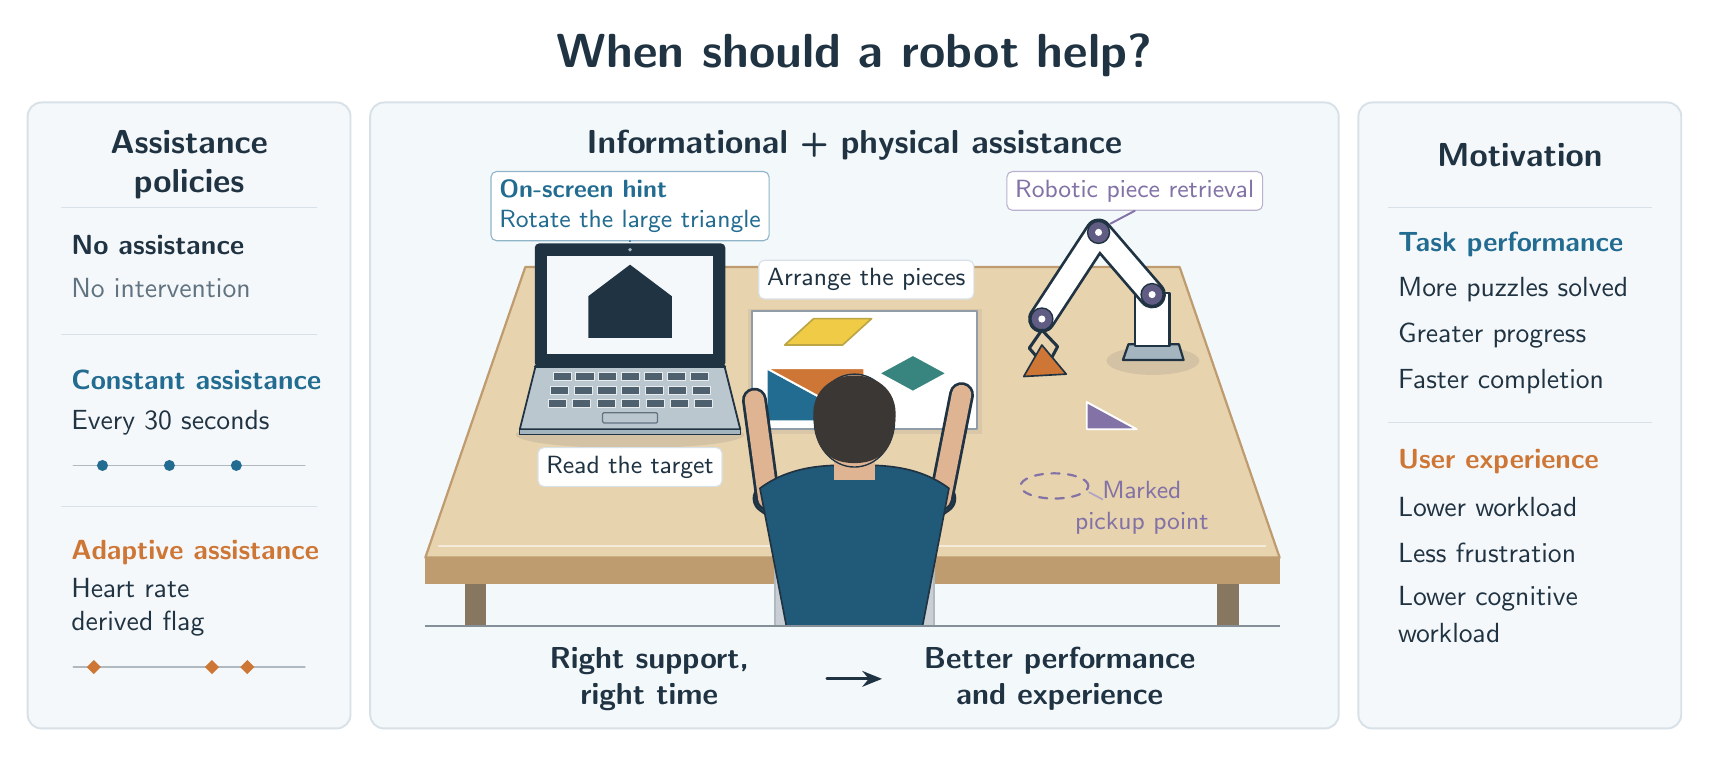
\begin{tikzpicture}[
  x=1cm,y=1cm,line cap=round,line join=round,
  font=\sffamily\fontsize{11}{13}\selectfont,text=ink,
  title/.style={font=\sffamily\bfseries\fontsize{13}{15}\selectfont},
  small/.style={font=\sffamily\fontsize{10}{12}\selectfont},
  tinylabel/.style={font=\sffamily\fontsize{9}{11}\selectfont},
  card/.style={draw=line,fill=wash,rounded corners=5pt,line width=.7pt},
  chip/.style={draw=line,fill=white,rounded corners=2pt,inner sep=3pt,
    font=\sffamily\fontsize{9}{11}\selectfont},
  arrow/.style={-{Stealth[length=2.5mm,width=2mm]},draw=muted,line width=.8pt}
]
\path[use as bounding box] (0,1.05) rectangle (21,10.0);
\node[title,font=\sffamily\bfseries\fontsize{18}{20}\selectfont]
  at (10.5,9.65) {When should a robot help?};

% Original composition: task sidebar, central perspective scene, outcome sidebar.
\draw[card] (0,1.10) rectangle (4.10,9.05);
\draw[card,fill=bluewash!55!white] (4.35,1.10) rectangle (16.65,9.05);
\draw[card] (16.90,1.10) rectangle (21,9.05);
\node[title,font=\sffamily\bfseries\fontsize{12}{14}\selectfont,
  anchor=north,align=center,text width=3.2cm,inner sep=0pt]
  at (2.05,8.70) {Assistance\\policies};
\draw[draw=line] (.43,7.72) -- (3.67,7.72);
% Three vertically aligned policy entries; dots are illustrative, not event logs.
\node[small,font=\sffamily\bfseries\fontsize{10}{12}\selectfont,
  anchor=west] at (.43,7.24) {No assistance};
\node[small,anchor=west,text=muted] at (.43,6.69) {No intervention};
\draw[draw=line] (.43,6.10) -- (3.67,6.10);
\node[small,font=\sffamily\bfseries\fontsize{10}{12}\selectfont,
  anchor=west,text=blue] at (.43,5.53) {Constant assistance};
\node[small,anchor=west] at (.43,4.98) {Every 30 seconds};
\draw[draw=muted!50,line width=.6pt] (.58,4.44) -- (3.52,4.44);
\foreach \x in {.95,1.80,2.65}{\fill[blue] (\x,4.44) circle (.07);}
\draw[draw=line] (.43,3.92) -- (3.67,3.92);
\node[small,font=\sffamily\bfseries\fontsize{10}{12}\selectfont,
  anchor=west,text=orange] at (.43,3.34) {Adaptive assistance};
\node[small,anchor=west,align=left] at (.43,2.64)
  {Heart rate\\derived flag};
\draw[draw=muted!50,line width=.6pt] (.58,1.88) -- (3.52,1.88);
\foreach \x in {.84,2.34,2.79}{
  \fill[orange] (\x,1.97) -- (\x+.09,1.88)
    -- (\x,1.79) -- (\x-.09,1.88) -- cycle;
}

% Perspective tabletop: a narrower far edge and a visible front fascia.
\node[title,font=\sffamily\bfseries\fontsize{12}{14}\selectfont,
  anchor=north,inner sep=0pt] at (10.50,8.70)
  {Informational + physical assistance};
% Clip the scene at a straight lower edge; there is no floor-shadow oval.
\begin{scope}
\clip (4.35,2.40) rectangle (16.65,8.30);
\fill[woodedge] (5.05,2.93) -- (15.90,2.93) -- (15.90,3.27) -- (5.05,3.27) -- cycle;
\filldraw[fill=wood,draw=woodedge,line width=.8pt]
  (5.05,3.27) -- (15.90,3.27) -- (14.63,6.96) -- (6.32,6.96) -- cycle;
\draw[draw=white!55!wood,line width=.6pt] (5.22,3.42) -- (15.72,3.42);
\fill[woodedge!65!ink] (5.55,2.25) rectangle (5.82,2.93);
\fill[woodedge!65!ink] (15.11,2.25) rectangle (15.38,2.93);

% Unrotated puzzle block, moved toward the participant; not a scored puzzle.
\begin{scope}[shift={(9.20,4.90)},x={(.92cm,0cm)},y={(0cm,.50cm)}]
  \fill[ink,opacity=.07] (-.05,-.12) -- (3.18,-.12)
    -- (3.18,3.05) -- (-.05,3.05) -- cycle;
  \filldraw[fill=white,draw=muted!70,line width=.8pt]
    (0,0) -- (3.10,0) -- (3.10,3.0) -- (0,3.0) -- cycle;
  \filldraw[fill=blue,draw=white,line width=.7pt]
    (.20,.20) -- (1.55,.20) -- (.20,1.55) -- cycle;
  \filldraw[fill=orange,draw=white,line width=.7pt]
    (1.55,.20) -- (1.55,1.55) -- (.20,1.55) -- cycle;
  \filldraw[fill=teal,draw=white,line width=.7pt]
    (2.22,.95) -- (2.69,1.42) -- (2.22,1.89) -- (1.75,1.42) -- cycle;
  \filldraw[fill=yellow,draw=ink!25!yellow,line width=.6pt]
    (.45,2.14) -- (1.25,2.14) -- (1.65,2.81) -- (.85,2.81) -- cycle;
\end{scope}
% Loose purple triangle below the robot base, clear of the pickup marker.
\filldraw[fill=purple,draw=white,line width=.7pt]
  (13.45,4.90) -- (14.085,4.90) -- (13.45,5.245) -- cycle;
\node[chip] at (10.65,6.80) {Arrange the pieces};

% Laptop: centered rectangular display and symmetric, widening keyboard plane.
% Both halves share the same horizontal hinge; there is no lateral shear.
\fill[ink,opacity=.10] (7.65,4.83) ellipse (1.45 and .17);
\filldraw[fill=metal!75!white,draw=ink,line width=.65pt]
  (6.25,4.90) -- (9.05,4.90) -- (8.85,5.70) -- (6.45,5.70) -- cycle;
\filldraw[fill=metal,draw=ink,line width=.5pt]
  (6.25,4.90) -- (9.05,4.90) -- (9.05,4.83) -- (6.25,4.83) -- cycle;
\foreach \y/\left/\step in {5.52/6.67/.29,5.35/6.64/.30,5.18/6.61/.31}{
\foreach \i in {0,...,6}{
  \filldraw[fill=ink!65!metal,draw=white!75!metal,line width=.2pt]
    ({\left+\i*\step},\y) rectangle ({\left+\i*\step+.23},\y+.10);
}}
\draw[draw=muted,line width=.45pt,rounded corners=.5pt]
  (7.30,4.98) rectangle (8.00,5.11);
\draw[draw=ink,line width=1.2pt] (6.45,5.70) -- (8.85,5.70);
\filldraw[fill=ink,draw=ink,line width=.55pt,rounded corners=1.3pt]
  (6.45,5.70) rectangle (8.85,7.25);
\fill[wash] (6.60,5.86) rectangle (8.70,7.10);
\fill[metal] (7.65,7.18) circle (.025);
% Black silhouette remains the target, not a colored solution.
\fill[ink] (7.12,6.06) -- (8.18,6.06) -- (8.18,6.59)
  -- (7.65,6.99) -- (7.12,6.59) -- cycle;
\node[chip] at (7.65,4.42) {Read the target};

% Text hint above its screen, avoiding a second competing display.
\node[chip,draw=blue!50,fill=white,align=left,text=blue,anchor=north,
  font=\sffamily\fontsize{9}{11}\selectfont] (hint) at (7.65,8.18)
  {\textbf{On-screen hint}\\Rotate the large triangle};
\draw[draw=blue,line width=.7pt] (hint.south) -- (7.65,7.29);

% Marked pickup point and simplified articulated robot on the table's right.
% Shift the entire footprint inward: its furthest corner is inside the table.
\begin{scope}[shift={(-.60,0)}]
\draw[draw=purple,line width=.8pt,dashed]
  (13.64,4.18) ellipse (.43 and .16);
\node[tinylabel,text=purple,align=center] at (14.75,3.90) {Marked\\pickup point};
\draw[draw=purple!65,line width=.6pt] (14.08,4.10) -- (14.25,4.01);
\fill[ink,opacity=.10] (14.89,5.77) ellipse (.59 and .18);
\filldraw[fill=metal,draw=ink,line width=.8pt]
  (14.51,5.78) -- (15.28,5.78) -- (15.22,5.98) -- (14.58,5.98) -- cycle;
\filldraw[fill=white,draw=ink,line width=.8pt]
  (14.66,5.96) rectangle (15.10,6.63);
\draw[draw=ink,line width=10pt] (14.88,6.61) -- (14.20,7.40) -- (13.48,6.30);
\draw[draw=white,line width=8pt] (14.88,6.61) -- (14.20,7.40) -- (13.48,6.30);
\foreach \x/\y in {14.88/6.61,14.20/7.40,13.48/6.30}{
  \filldraw[fill=purple!65!ink,draw=ink,line width=.5pt] (\x,\y) circle (.14);
  \fill[white] (\x,\y) circle (.045);
}
\draw[draw=ink,line width=1.1pt]
  (13.48,6.16) -- (13.32,5.93) -- (13.45,5.78);
\draw[draw=ink,line width=1.1pt]
  (13.48,6.16) -- (13.68,5.95) -- (13.59,5.78);
\filldraw[fill=orange,draw=ink,line width=.6pt]
  (13.25,5.57) -- (13.79,5.60) -- (13.48,5.97) -- cycle;
\node[chip,draw=purple!55,text=purple,anchor=north] (retrieval)
  at (14.66,8.18) {Robotic piece retrieval};
\draw[draw=purple,line width=.7pt] (retrieval.south) -- (14.35,7.51);
\end{scope}

% Centered seated participant, seen from behind.
% Painter's order is deliberate: chair, arms, torso, neck, then head.
% The back masks proximal upper arms; only elbows and reaching forearms show.
\filldraw[fill=muted!35,draw=muted!50,line width=.6pt,rounded corners=4pt]
  (9.49,2.03) rectangle (11.51,3.96);
% Left and right upper arms originate behind the torso's shoulder silhouette.
\draw[draw=ink,line width=11pt] (9.82,3.72) -- (9.40,4.02);
\draw[draw=blue,line width=9pt] (9.82,3.72) -- (9.40,4.02);
\draw[draw=ink,line width=9pt] (9.40,4.02) -- (9.23,5.27);
\draw[draw=skin,line width=7pt] (9.40,4.02) -- (9.23,5.27);
\draw[draw=ink,line width=11pt] (11.18,3.72) -- (11.60,4.02);
\draw[draw=blue,line width=9pt] (11.18,3.72) -- (11.60,4.02);
\draw[draw=ink,line width=9pt] (11.60,4.02) -- (11.86,5.34);
\draw[draw=skin,line width=7pt] (11.60,4.02) -- (11.86,5.34);
% Back drawn over the arm roots, not underneath them.
\filldraw[fill=blue!70!ink,draw=ink,line width=.6pt]
  (9.67,2.22) -- (11.33,2.22) -- (11.70,4.15)
  .. controls (11.38,4.39) and (11.01,4.43) .. (10.78,4.44)
  -- (10.22,4.44)
  .. controls (9.99,4.43) and (9.62,4.39) .. (9.30,4.15) -- cycle;
\fill[skin] (10.24,4.25) rectangle (10.76,4.68);
\filldraw[fill=skin,draw=ink,line width=.5pt] (10.50,5.01) ellipse (.51 and .59);
\fill[hair] (9.99,4.96)
  .. controls (9.83,5.79) and (11.17,5.79) .. (11.01,4.96)
  .. controls (10.98,4.58) and (10.75,4.47) .. (10.50,4.47)
  .. controls (10.25,4.47) and (10.02,4.58) .. cycle;
\end{scope}
% Short inset boundary clips only the artwork, leaving space for the motivation.
\draw[draw=ink!55,line width=.8pt,line cap=butt] (5.05,2.40) -- (15.90,2.40);
\node[font=\sffamily\bfseries\fontsize{11}{13}\selectfont,
  anchor=east,align=center,text width=4.2cm,inner sep=0pt] at (10.00,1.73)
  {Right support,\\right time};
\draw[arrow,draw=ink,line width=1pt] (10.15,1.73) -- (10.85,1.73);
\node[font=\sffamily\bfseries\fontsize{11}{13}\selectfont,
  anchor=west,align=center,text width=4.2cm,inner sep=0pt] at (11.00,1.73)
  {Better performance\\and experience};

% Aspirational benefits motivate the study; these are not empirical effect claims.
\node[title,font=\sffamily\bfseries\fontsize{12}{14}\selectfont,
  anchor=center,align=center,text width=3.2cm,inner sep=0pt]
  at (18.95,8.385) {Motivation};
\draw[draw=line] (17.28,7.72) -- (20.62,7.72);
\node[small,font=\sffamily\bfseries\fontsize{10}{12}\selectfont,text=blue,
  anchor=west] at (17.28,7.24) {Task performance};
\node[small,anchor=west] at (17.28,6.67) {More puzzles solved};
\node[small,anchor=west] at (17.28,6.09) {Greater progress};
\node[small,anchor=west] at (17.28,5.51) {Faster completion};
\draw[draw=line] (17.28,4.99) -- (20.62,4.99);
\node[small,font=\sffamily\bfseries\fontsize{10}{12}\selectfont,text=orange,
  anchor=west] at (17.28,4.49) {User experience};
\node[small,anchor=west] at (17.28,3.91) {Lower workload};
\node[small,anchor=west] at (17.28,3.33) {Less frustration};
\node[small,anchor=west] at (17.28,2.75) {Lower cognitive};
\node[small,anchor=west] at (17.28,2.32) {workload};

\end{tikzpicture}%
}
\end{document}
